\section{Caracterización de la red actual}
\label{sec:caracterizacion}

La red considerada para el comienzo de este proyecto consiste en un
tendido de fibra óptica estándar tipo G.652.D (ver sección
\ref{sec:marcoteorico}). Cada enlace de fibra óptica une un par de
\emph{DC} de forma directa y sin estaciones intermedias mediante
cables de 96 fibras diseñadas para operar en la banda C. Esta red no
posee ningún tipo de multiplexor. En un comienzo, cada fibra tiene
soporte para un solo servicio usando un par de transmisión y recepción
Láser, filtros y amplificadores, donde aplique. Se supone, sin
embargo, que en un comienzo el tendido de fibras es de un punto a otro
entre dos \emph{DC}, sin ningún tipo de equipos instalado.

El tendido inicial es de 399 Km distribuídos en 9 tramos, de los
cuales tres son de distancias mayores a 40 Km. Este tendido tal y como
está no tiene considerado ningún análisis que considere cortes de los
cables, por lo que no existen garantías \emph{SLA} que establezcan
políticas claras de calidad de servicio. Por otro lado, es sabido que
tramos de más de 30 Km. deben ser compensados en atenuación y los
mayores a 40 Km. deben ser compensados en dispersión
cromática. También por esa razón el tendido de fibra oscura no cumple
con el \emph{SLA} establecido en calidad de la señal debido a que no
existen garantías de una correcta recepción de la señal.

Por otro lado, no existen en la red inicial mecanismos íntegros de
recepción, tales cómo equipos de \textit{Optical Distribution Frame
  (ODF)}, equipos Mux/Demux (\textit{ROADM/WSS}) con sus respectivos
\textit{racks} y \textit{shelves}, por lo que la red no resulta
escalable en equipamiento tampoco.

Las aplicaciones de la red actual son limitadas, pero igualmente
tienen algún sentido. Las redes oscuras son una forma precaria pero
rápida de interconectar dos nodos. Si es necesario conectar dos
\emph{DC} a través de un nodo intermedio, un enlace físico debe ser
establecido para que ello ocurra. No hay detalles sobre cómo se
interconectaban los nodos ``discontinuos'', solo lo hay entre nodos
contiguos.

\begin{figure}[h]
\centering
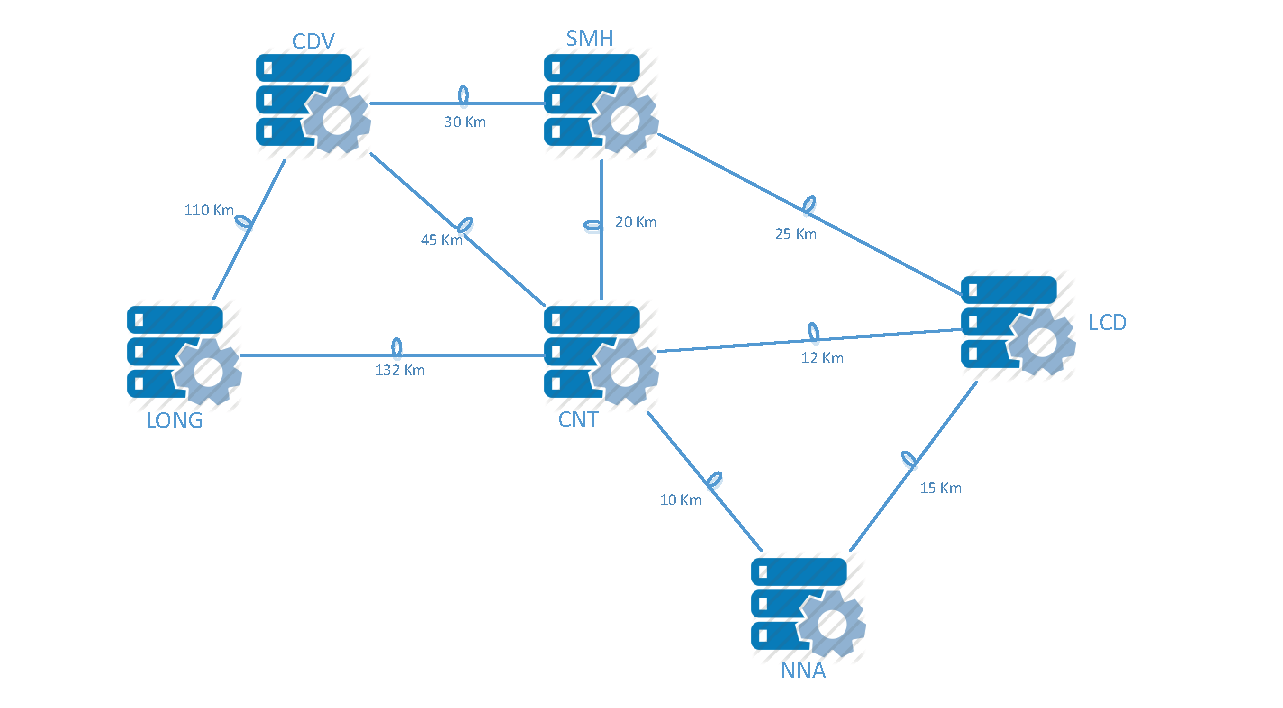
\includegraphics[width=0.8\textwidth]{Imagenes/Diagrama_Fibra_Oscura.eps}
\caption{Diagrama inicial de red oscura preexistente. Este diagrama se
  presenta a los distintos proveedores para poder estimar el
  número necesario de amplificadores, compensadores de dispersión,
  etcétera.}
\label{fig:diagrama_red}
\end{figure}

% Para la caracterización y planificación de la red, se consideran 3
% factores claves en todas sus etapas:

% \begin{itemize}
% \item Delay Introducido
% \item Distancia
% \item Costos Monetarios
% \end{itemize}

% Para la Fibra Oscura:

% Si el delay es considerado, se puede incluir cómo un costo adicional
% de distancia (sabiendo la relación entre cantidad de saltos y
% distancia), de tal forma que la minimización ocurra en torno a una
% sola variable.

% Una vez resueltos los costos en una sola variable (Saltos y
% Distancia), se procederá a minimizar la función costo usando el
% conocido algoritmo de Dijkstra.

% Adicionalmente a este procedimiento, para el caso de posibles cortes
% simultáneos, ha de hacerse un estudio probabilístico, dependiendo de
% que tan probable es que se corte una fibra según un umbral ``$\mu$'' se
% dispondrá de una o más rutas alternativas para esta.
